\documentclass[a4paper,11pt]{article}

% ---------- Packages ----------
\usepackage[margin=2.5cm]{geometry}
\usepackage{amsmath, amssymb, amsthm, mathtools}
\usepackage{algorithm}
\usepackage{algpseudocode}
\usepackage{enumitem}
\usepackage{graphicx}
\usepackage{booktabs}
\usepackage{hyperref}
\usepackage{xcolor}

\usepackage{tikz}
\usetikzlibrary{automata,positioning,arrows.meta}

% ---------- Theorem Environments ----------
\newtheorem{theorem}{Theorem}
\newtheorem{lemma}{Lemma}
\newtheorem{definition}{Definition}
\newtheorem{proposition}{Proposition}
\newtheorem{corollary}{Corollary}

% ---------- Custom Commands ----------
\newcommand{\R}{\mathbb{R}}
\newcommand{\N}{\mathbb{N}}
\newcommand{\Z}{\mathbb{Z}}
\newcommand{\Alphabet}{\Sigma}
\newcommand{\eps}{\varepsilon}
\newcommand{\set}[1]{\left\{ #1 \right\}}
\newcommand{\abs}[1]{\left| #1 \right|}
\newcommand{\ceil}[1]{\left\lceil #1 \right\rceil}
\newcommand{\floor}[1]{\left\lfloor #1 \right\rfloor}

% ---------- Section Style ----------
\renewcommand{\thesubsection}{(\alph{subsection})}
\renewcommand{\thesection}{}

% ---------- Algorithm Style ----------
\algrenewcommand\algorithmicrequire{\textbf{Input:}}
\algrenewcommand\algorithmicensure{\textbf{Output:}}

% ---------- Title Info ----------
\title{\textbf{CSE2315 --- Assignment 6}}
\author{Vlad Paun \\ 6152937}
\date{\today}

% ---------- Document ----------
\begin{document}

	\maketitle

	\section{Exercise 1}
	Suppose we have the following language:
	\[
	E_{\mathrm{GNFA}} = \set{\langle G \rangle \mid G \text{ is a GNFA such that } L(G)=\emptyset }.
	\]

	Show that $E_{\mathrm{GNFA}}$ is decidable. You are allowed to make use of the deciders implied by the text in the book (e.g., Section 4.1).

	\vspace{1cm}

	\section{Exercise 2}
	Consider the language
	\[
	L = \set{\langle M,w \rangle \mid M \text{ halts on } w \text{ and moves the head at most } |w|^2 \text{ steps}}.
	\]

	Is this language decidable? Explain.

	\vspace{1cm}

	\section{Exercise 3}
	Old exam question, endterm 20--21: Show the claim is true or give a counterexample and explanation to show the claim is false, starting your answer with either \textbf{True} or \textbf{False}.

	If there is a Turing reduction from $L$ to $E_{\mathrm{CFG}}$, then $\overline{L}$ is Turing-recognisable.

	\vspace{1cm}

	\section{Exercise 4}
	Old exam question, endterm 22--23:

	Consider the following language:
	\[
	L = \set{\langle M,q \rangle \mid M \text{ is a Turing Machine and } q \text{ is a useless state in } M }.
	\]

	A useless state in a Turing Machine is one that is never entered on any input string.

	Prove $L$ is undecidable, using a Turing reduction $E_{\mathrm{TM}} \leq_T L$.

	\vspace{1cm}

	\section{Exercise 5}
	Old exam question, resit 17--18: Suppose we have the following language
	\begin{align*}
	L = \{\langle M,v,G \rangle \mid & M \text{ outputs } G \text{ on the tape, which is a context free grammar}\\
	&\text{that accepts } v,\text{ when run on input } v.\}
	\end{align*}

	We intend to prove that this language is undecidable. To that end we use a mapping reduction from $HALT_{TM}$ to $L$. The reduction $f$ is computed by the following TM $F$:

	\begin{quote}
		$F =$ ``On input $\langle M,w \rangle$:
		\begin{enumerate}[label=\arabic*.]
			\item Construct the following TM $M'$:
			\begin{quote}
				$M' =$ ``On input $x$:
				\begin{enumerate}[label=\arabic*.]
					\item Clear the input from the tape.
					\item Run $M$ on $w$.
					\item See question a.
					\item See question a.
				\end{enumerate}
				''
			\end{quote}
			\item Write $\langle M',a,G \rangle$ to the output tape, where $G$ is a grammar with one rule: $S \to a$ and starting variable $S$.''
		\end{enumerate}
	\end{quote}

	\subsection{What should be done in steps 3 and 4 of $M'$?}

	\vspace{1cm}

	\subsection{Provide a proof showing $f$ satisfies the requirements of a mapping reduction.}

	\vspace{1cm}

	\section{Exercise 6}
	Old exam question, resit 20--21:

	\subsection{Let $MIA_{TM}$ be the language consisting of 3 TM's and a word such that the word is recognized by at least 2 of the 3 TM's. Show that this is a recognizable language.}
	Formally described as
	\begin{align*}
	MIA_{TM} = \{\langle M_1,M_2,M_3,w \rangle &\mid M_1,M_2,M_3 \text{ are TM's and }\\
	& w \in (L(M_1)\cap L(M_2)) \cup (L(M_1)\cap L(M_3)) \cup (L(M_2)\cap L(M_3)) \}.
	\end{align*}

	\vspace{1cm}

	\subsection{Show that $MIA_{TM}$ is undecidable by constructing a Turing reduction from $A_{TM}$.}

	\vspace{1cm}

	\subsection{Show that $MIA_{TM}$ is not co-Turing recognizable.}

	\vspace{1cm}

	\section{Exercise 7}
	Revision, old exam question, midterm 19--20: Assume that we define an expanded NFA model by imposing the additional requirement that $|F|=1$, and we call this an SNFA.

	\subsection{ Are the SNFA and NFA models equally expressive?}
	Start your answer with ``Yes'' or ``No''. If you answer yes, explain how an arbitrary SNFA can be rewritten as an NFA and vice versa. If you answer no, give an example of a language that can be accepted by an NFA, but not by an SNFA or vice versa.

	\vspace{1cm}

	\subsection{Give an NFA of at most 4 states that accepts the word \texttt{mia} and rejects the word \texttt{maya}. No other restrictions on the language apply. A transition diagram suffices.}

	\vspace{1cm}

	\subsection{Consider the NFA $N$ depicted as:}

	\begin{center}
		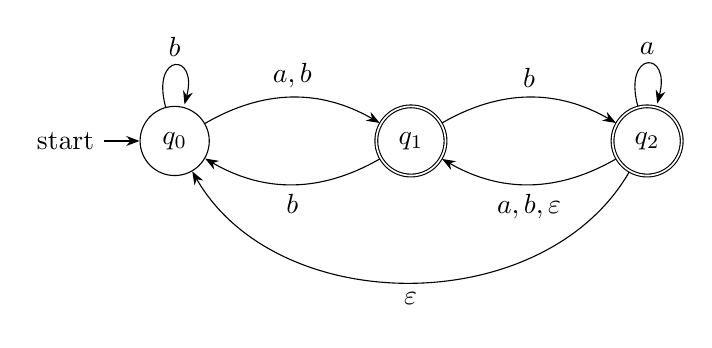
\begin{tikzpicture}[->, >=Stealth, auto, node distance=3cm]
			\node[initial,state] (q0) {$q_0$};
			\node[state, accepting] (q1) [right of=q0] {$q_1$};
			\node[state,accepting] (q2) [right of=q1] {$q_2$};

			\path
			(q0) edge[loop above] node {$b$} (q0)
			(q0) edge[bend left] node {$a,b$} (q1)
			(q1) edge[bend left] node {$b$} (q0)
			(q1) edge[bend left] node {$b$} (q2)
			(q2) edge[loop above] node {$a$} (q2)
			(q2) edge[bend left] node[below] {$a,b,\eps$} (q1)
			(q2) edge[bend left=60] node[below] {$\eps$} (q0);
		\end{tikzpicture}
	\end{center}

	Using the method from Sipser and leaving out unreachable states, construct a new DFA $D$, such that $L(D)=L(N)$. A transition diagram and a short explanation suffice.

\end{document}